\documentclass[10pt, aspectratio=169]{beamer} %
\usetheme{Singapore}

\usepackage{bookmark}
\usepackage{graphicx}
\usepackage[english]{babel}
\usepackage[utf8]{inputenc}
\usepackage[T1]{fontenc}
\usepackage{amsmath}
\usepackage{color}
\usepackage{listings}
\usepackage{tabularx}
\usepackage{amssymb}
\usepackage{lmodern}

\usepackage{hyperref}
\hypersetup{colorlinks=true, urlcolor=blue}

\DeclareMathOperator*{\minimize}{minimize} %in preamble
 
\newcommand{\N}{{\mathbb{N}}}
\newcommand{\I}{{\bf I}}
\newcommand{\C}{{\bf C}}
\newcommand{\A}{{\bf A}}
\newcommand{\T}{{\bf T}}
\newcommand{\g}{{\bf g}}
\newcommand{\e}{{\bf e}}
\newcommand{\ab}{{\bf a}}
\newcommand{\ba}{{\bf b}}
\newcommand{\Z}{{\mathbb{Z}}}
\newcommand{\R}{{\mathbb{R}}}
\newcommand{\mbf}{\mathbf}
\newcommand{\bs}{\boldsymbol}
\newcommand{\cc}{{\bf c}}
\newcommand{\su}{{\sum_{n=0}^{N-1}}}

\newcommand{\argmax}{\mathop{\text{arg\;max}}}
\newcommand{\argmin}{\mathop{\text{arg\;min}}}

\newcommand{\HH}{{\bf H}}
\newcommand{\thb}{\boldsymbol{\theta}}
\newcommand{\w}{{\bf w}}
\newcommand{\Sigb}{\boldsymbol{\Sigma}}
\newcommand{\mub}{\boldsymbol{\mu}}
\newcommand{\alb}{\boldsymbol{\alpha}}

\newcommand{\s}{{\bf s}}
\newcommand{\SB}{{\bf S}}

\definecolor{blue}{RGB}{32,32,255}
\graphicspath{{./images/}}

\newcommand{\h}{{\bf h}}
\newcommand{\rr}{{\bf r}}
\newcommand{\X}{{\bf X}}
\newcommand{\x}{{\bf x}}
\newcommand{\y}{{\bf y}}
\newcommand{\p}{{\bf p}}
\newcommand{\E}{{\bf E}}
\newcommand{\U}{{\bf U}}
\newcommand{\V}{{\bf V}}
\newcommand{\f}{{\bf f}}
\newcommand{\var}{{\mathop{\text{var}}}}

\newcommand{\F}{{\cal F}}
\newcommand{\leveys}{0.75\textwidth}
\newcommand{\etaisyys}{0.25\textwidth}

\newcommand{\sinc}{\mathop{\text{sinc}}}
\newcommand{\esim}{\em}

\newcommand{\modulo}{\operatorname{mod}}

\setbeamertemplate{frametitle continuation}[from second] 

\renewcommand{\insertcontinuationtext}{}

\setbeamertemplate{frametitle}
{
	\vspace*{0.7cm} \vbox{\insertframetitle}
}

\usecolortheme{default}

\setbeamertemplate{mini frames}{}
\renewcommand*{\slideentry}[6]{}
\setbeamertemplate{frametitle}{
    \vspace*{0.2cm}
    \insertframetitle
}

\title{Pattern Recognition and Machine Learning}
\subtitle{Slide Set 3: Detection Theory}
\author{Heikki Huttunen\\
heikki.huttunen@tuni.fi}
\institute{Signal Processing\\Tampere University}
\date{October 2020}

\begin{document}

\maketitle

\lstdefinestyle{mystyle}{
  belowcaptionskip=1\baselineskip,
  breaklines=true,
  frame=single,
  xleftmargin=\parindent,
  language=Python,
  showstringspaces=false,
  basicstyle=\tiny\ttfamily,
  keywordstyle=\bfseries\color{green!40!black},
  commentstyle=\itshape\color{purple!40!black},
  identifierstyle=\color{blue},
  stringstyle=\color{orange},
  moredelim=**[is][\color{red}]{@}{@},
}

\lstset{language=Python,style=mystyle} 

\begin{frame}[allowframebreaks=0.8]
 {Detection theory}
\begin{itemize}
\item In this section, we will briefly consider
detection theory.
\item Detection theory has many common topics with machine learning.
\item The methods are based on estimation theory and attempt
to answer questions such as
\begin{itemize}
\item Is a signal of specific model present in our time series?
E.g., detection of noisy sinusoid; beep or no beep?
\item Is the transmitted pulse present at radar signal at time $t$?
\item Does the mean level of a signal change at time $t$?
\item After calculating the mean change in pixel values of subsequent
frames in video, is there something moving in the scene?
\item Is there a person in this video frame?
\end{itemize}
\item The area is closely related to \emph{hypothesis testing}, which
is widely used e.g., in medicine: Is the response in patients due
to the new drug or due to random fluctuations?
\item Consider the detection of a sinusoidal waveform
\end{itemize}
\centerline{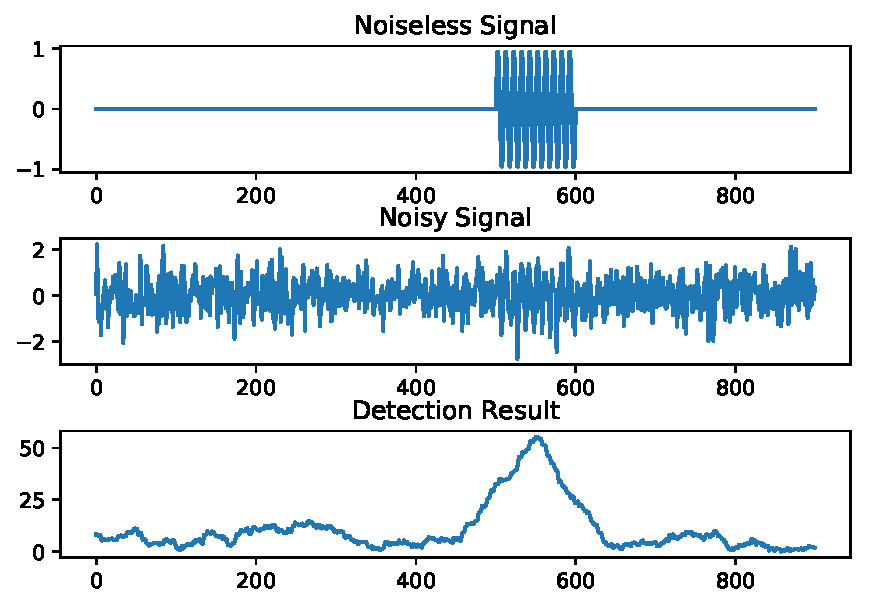
\includegraphics[width=0.4\textwidth]{rayleighSinusoid.pdf}}
\end{frame}

\begin{frame}[allowframebreaks=0.8]
 {Detection theory}
\begin{itemize}
\item In our case, the hypotheses could be
\begin{align*}
{\cal H}_1 &: x[n] = A \cos(2\pi f_0 n + \phi) + w[n]\\
{\cal H}_0 &: x[n] = w[n]
\end{align*}
\item This example corresponds to detection of noisy sinusoid.
\item The hypothesis ${\cal H}_1$ corresponds to the case that the sinusoid
is present and is called \emph{alternative hypothesis}.
\item The hypothesis ${\cal H}_0$ corresponds to the case that the measurements
consists of noise only and is called \emph{null hypothesis}.
\end{itemize}
\end{frame}

\begin{frame}[allowframebreaks=0.8]
 {Introductory Example}
\begin{itemize}
%\item \emph{Neyman-Pearson approach} is the classical way of solving 
%detection problems in an optimal manner. 
%\item It relies on so called \emph{Neyman-Pearson theorem}.
\item Consider a simplistic detection
problem, where we observe one sample $x[0]$ from one of two
densities: ${\cal N}(0,1)$ or ${\cal N}(1,1)$. 
\item The task is to choose the correct density in an optimal manner.


\centerline{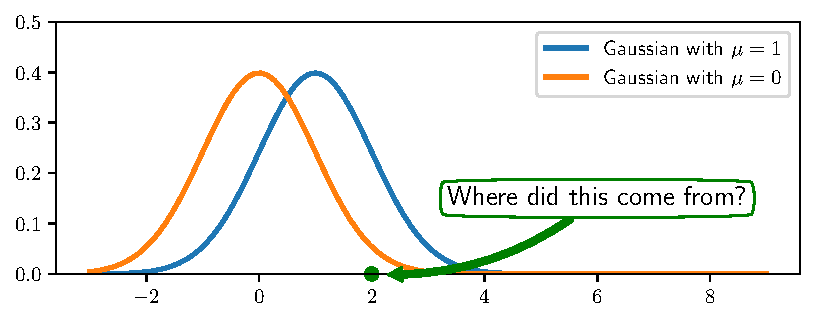
\includegraphics[width=0.6\textwidth]{two_gaussians.pdf}}
\eject

\item Our hypotheses are now
\begin{align*}
{\cal H}_1 &: \mu = 1,\\
{\cal H}_0 &: \mu = 0,
\end{align*}
and the corresponding likelihoods are plotted below.

\end{itemize}
\centerline{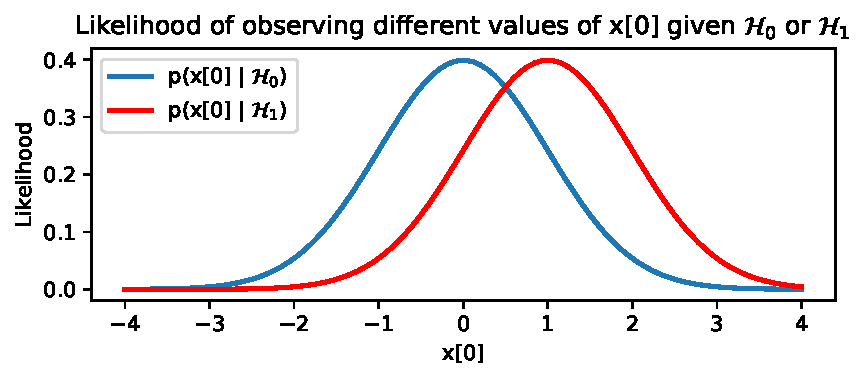
\includegraphics[width=0.5\textwidth]{NeymanPearson.pdf}}

\begin{itemize}

\item An obvious approach for deciding the density would choose
the one, which is higher for a particular $x[0]$.
\item More specifically, study the likelihoods and choose the more likely one.
\item The likelihoods are
\begin{align*}
{\cal H}_1 &: p(x[0]\mid \mu=1) =  \frac{1}{\sqrt{2\pi}}\exp\left(-\frac{(x[0]-1)^2}{2}\right).\\
{\cal H}_0 &: p(x[0]\mid \mu=0) =  \frac{1}{\sqrt{2\pi}}\exp\left(-\frac{(x[0])^2}{2}\right).
\end{align*}
\item One should select ${\cal H}_1$ if "$\mu = 1$" is more likely than "$\mu = 0$".
\item In other words, $p(x[0]\mid \mu=1) > p(x[0]\mid \mu=0)$.
\item Let's state this in terms of $x[0]$:
\begin{align*}
&\; p(x[0]\mid \mu=1) > p(x[0]\mid \mu=0) \\
\Leftrightarrow &\; \frac{p(x[0]\mid \mu=1)}{p(x[0]\mid \mu=0)} > 1\\
\Leftrightarrow &\; \frac{\frac{1}{\sqrt{2\pi}}\exp\left(-\frac{(x[0]-1)^2}{2}\right)}{\frac{1}{\sqrt{2\pi}}\exp\left(-\frac{(x[0])^2}{2}\right)} > 1\\
\Leftrightarrow &\; \exp\left(-\frac{(x[0]-1)^2 - x[0]^2}{2}\right) > 1
\end{align*}
\framebreak
\begin{align*}
\Leftrightarrow &\; (x[0]^2 - (x[0]-1)^2) > 0\\
\Leftrightarrow &\; 2x[0] - 1 > 0\\
\Leftrightarrow &\; x[0] > \frac12.
\end{align*}

\item In other words, choose ${\cal H}_1$ if $x[0] > 0.5$ and ${\cal H}_0$ if
$x[0] < 0.5$.

\item Studying the ratio of likelihoods (second row of the previous derivation)
is the key:
\[
\frac{p(x[0]\mid \mu=1)}{p(x[0]\mid \mu=0)} > 1
\]

\item This ratio is called \emph{likelihood ratio}, and comparison
to a threshold (here $\gamma = 1$) is called \emph{likelihood ratio test} (LRT).

\item Of course the \textit{detection threshold} $\gamma$ may be chosen other than $\gamma = 1$.

%\item Note, that it is also possible to study posterior probability ratios
%$p({\cal H}_1\mid \x) / p({\cal H}_0\mid \x)$ instead of the above likelihood
%ratio $p(\x\mid {\cal H}_1) / p(\x\mid {\cal H}_0)$. 
%\item However, using Bayes rule, this \emph{MAP test} turns out to be
%\[
%\frac{p(\x\mid {\cal H}_1)}{p(\x\mid {\cal H}_0)} > \frac{p({\cal H}_1)}{p(H_2)},
%\]
%i.e., the only effect of using posterior probability is on the 
%threshold for the LRT.
\end{itemize}
\end{frame}

%\begin{frame}[allowframebreaks=0.8]
% {Error Types}
%\begin{itemize}
%\item It might be that the detection problem is not symmetric and some
%errors are more costly than others.
%\item For example, when detecting a disease, a missed detection is more
%costly than a false alarm. 
%\item The tradeoff between misses and false alarms can be adjusted
%using the threshold of the LRT.
%\end{itemize}
%\end{frame}

\begin{frame}[allowframebreaks=0.8]
 {Error Types}
\begin{itemize}

\item The below figure illustrates the probabilities of the two kinds of
errors. 
\item The blue area on the left corresponds to the probability of
choosing ${\cal H}_1$ while ${\cal H}_0$ would hold (false match). 
\item 
The red area is the probability
of choosing  ${\cal H}_0$ while ${\cal H}_1$ would hold (missed detection).

\centerline{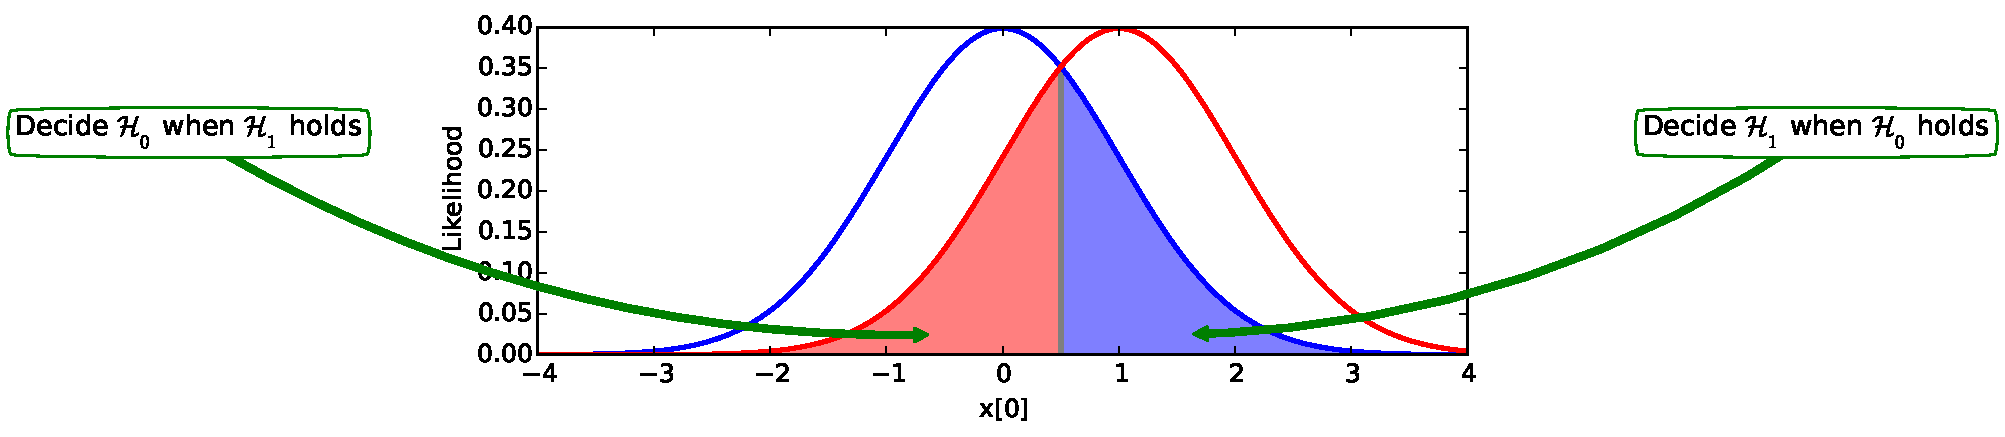
\includegraphics[width=\textwidth]{errorTypes1.pdf}}


\item It can be seen that we can decrease either probability arbitrarily small
by adjusting the detection threshold.

\begin{center}
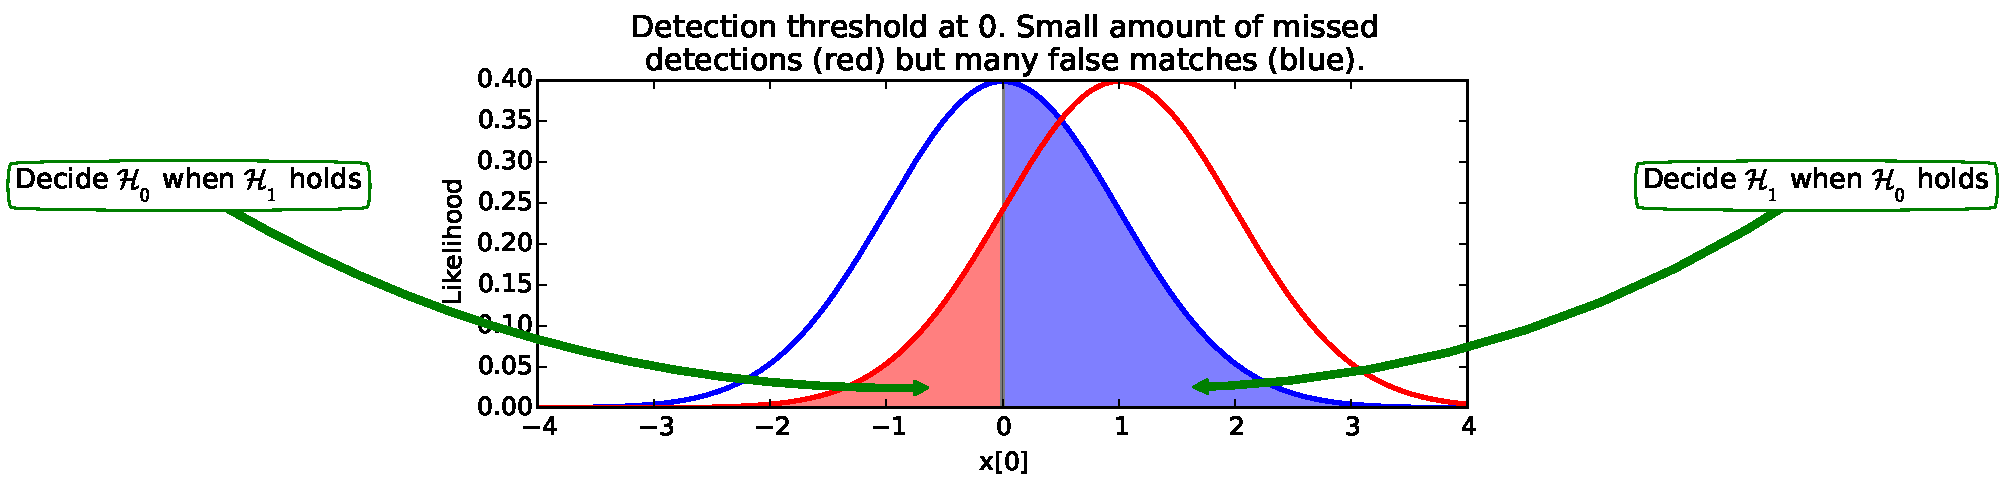
\includegraphics[width=0.65\textwidth]{errorTypes2.pdf}\\
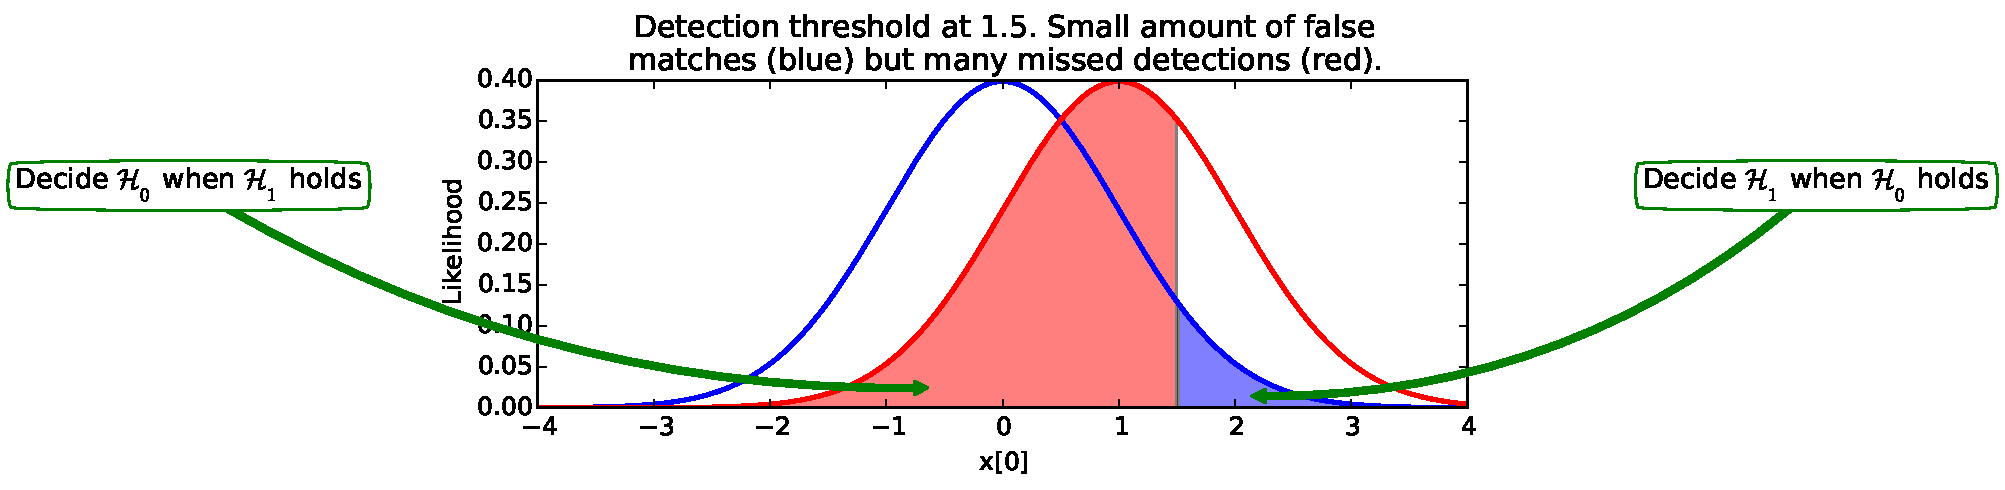
\includegraphics[width=0.65\textwidth]{errorTypes3.pdf}
\end{center}
\end{itemize}
\end{frame}

\begin{frame}[allowframebreaks=0.8]
 {Error Types}
\begin{center}
\includegraphics[width=10cm]{error_types.png}
\end{center}
{\tiny
\begin{itemize}
\item Picture from \url{https://en.wikipedia.org/wiki/Precision_and_recall}
\end{itemize}
}
\end{frame}

%\begin{frame}[allowframebreaks=0.8]
% {Error Types}
%\begin{itemize}
%{\small
%\item For example, suppose the threshold is $\gamma = 1.5$. What are $P_{FA}$ and $P_D$?
%\item Probability of false alarm is found by integrating over the blue area:
%\[
%P_{FA} = P(x[0]>\gamma \mid \mu = 0) = \int_{1.5}^{\infty} \frac{1}{\sqrt{2\pi}}\exp\left(-\frac{(x[0])^2}{2}\right)\,dx[0]\approx 0.0668.
%\]
%\item Probability of missed detection is the area marked in red:
%\[
%\hspace*{-0.7cm}
%P_{M} = P(x[0]<\gamma \mid \mu = 1) = \int_{-\infty}^{1.5} \frac{1}{\sqrt{2\pi}}\exp\left(-\frac{(x[0]-1)^2}{2}\right)\,dx[0] \approx 0.6915.
%\]
%\item An equivalent, but more useful term is the complement of $P_M$: probability of detection:
%\[
%P_{D} = 1 - P_M = \int_{1.5}^{\infty} \frac{1}{\sqrt{2\pi}}\exp\left(-\frac{(x[0]-1)^2}{2}\right)\,dx[0] \approx 0.3085.
%\]
%}
%\end{itemize}
%\end{frame}

%\begin{frame}[allowframebreaks=0.8]
% {Choosing the threshold}
%\begin{itemize}
%%\item Since $P_{FA}$ and $P_D$ depend on each other, we would like to maximize
%%$P_D$ subject to given maximum allowed $P_{FA}$. Luckily the following theorem makes this easy.
%%\item \textbf{Neyman-Pearson Theorem:} For a fixed $P_{FA}$, the likelihood ratio test
%%maximizes $P_D$ with the decision rule
%%\[
%%L(\x) = \frac{p(\x; {\cal H}_1)}{p(\x; {\cal H}_0)} > \gamma,
%%\]
%%with threshold $\gamma$ is the value for which
%%\[
%%\int_{\x:L(\x)>\gamma} p(\x; {\cal H}_0)\, d\x = P_{FA}.
%%\]
%%\framebreak
%%
%\item Often we don't want to define the threshold, but rather the amount of false alarms we can accept.
%\item For example, suppose we want to find the best detector for our
%introductory example, and we can tolerate 10\% false alarms ($P_{FA} = 0.1$).
%\item The likelihood ratio detection rule is:
%\[
%\text{Select } {\cal H}_1 \text{ if } \frac{p(x\mid \mu=1)}{p(x\mid \mu=0)} > \gamma
%\]
%The only thing to find out now is the threshold $\gamma$ such that
%\[
%\int_{\gamma}^{\infty} p(x\mid \mu=0)\, dx = 0.1.
%\]
%
%\end{itemize}
%\end{frame}
%
%\begin{frame}[allowframebreaks=0.8,fragile]
% {Choosing the threshold}
%
%\begin{itemize}
%\item This can be done with Python function \texttt{isf}, which solves
%the inverse cumulative distribution function.
%
%\begin{lstlisting}
%>>> import scipy.stats as stats
%
%>>> # Compute threshold such that P_FA = 0.1
%>>> T = stats.norm.isf(0.1, loc = 0, scale = 1)
%>>> print T
%1.28155156554
%\end{lstlisting}
%
%\item The parameters \verb+loc+ and \verb+scale+ are the mean and standard
%deviation of the Gaussian density, respectively.
%
%\end{itemize}
%
%\end{frame}

\begin{frame}[allowframebreaks=0.8]
 {Detector for a known waveform}
\begin{itemize}

%\item The NP approach applies to all cases where likelihoods are available.
\item An important special case is that of a known waveform $s[n]$ embedded in WGN sequence $w[n]$:
\begin{align*}
{\cal H}_1 &: x[n] = s[n] + w[n] \\
{\cal H}_0 &: x[n] = w[n].
\end{align*}
\item An example of a case where the waveform is known could be detection of radar 
signals, where a pulse $s[n]$ transmitted by us is reflected back after some 
propagation time.

\centerline{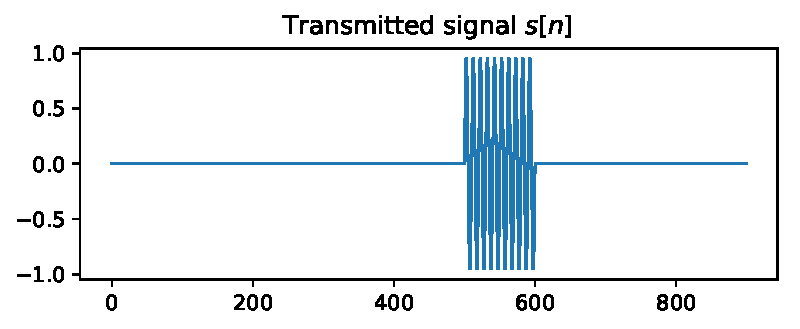
\includegraphics[width=0.4\textwidth]{clean_sinusoid.pdf} \quad 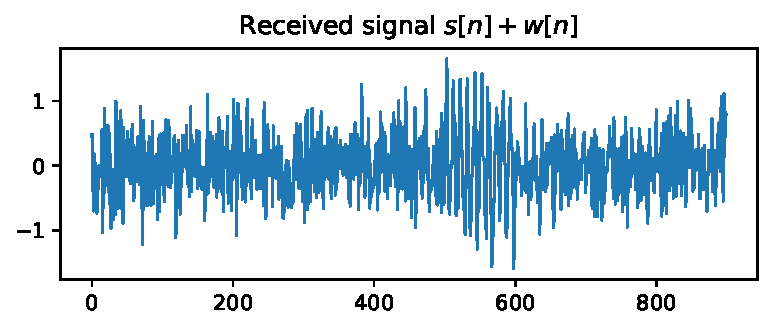
\includegraphics[width=0.4\textwidth]{noisy_sinusoid.pdf}}

\framebreak

\item For this case the likelihoods are
\begin{align*}
p(\x\mid {\cal H}_1) & =  \prod_{n=0}^{N-1}\frac{1}{\sqrt{2\pi\sigma^2}}\exp\left(-\frac{(x[n]-s[n])^2}{2\sigma^2}\right),\\
p(\x\mid {\cal H}_0) & =  \prod_{n=0}^{N-1}\frac{1}{\sqrt{2\pi\sigma^2}}\exp\left(-\frac{(x[n])^2}{2\sigma^2}\right).
\end{align*}
\item The likelihood ratio test is easily obtained as
\[
\hspace*{-0.5cm}
\frac{p(\x\mid {\cal H}_1)}{p(\x\mid {\cal H}_0)} = \exp\left[ -\frac{1}{2\sigma^2} \left( \sum_{n=0}^{N-1}(x[n]-s[n])^2 - \sum_{n=0}^{N-1}(x[n])^2 \right)\right] > \gamma.
\]
\item This simplifies by taking the logarithm from both sides:
\[
-\frac{1}{2\sigma^2} \left( \sum_{n=0}^{N-1}(x[n]-s[n])^2 - \sum_{n=0}^{N-1}(x[n])^2 \right) > \ln \gamma.
\]
\item This further simplifies into
\[
\frac{1}{\sigma^2} \sum_{n=0}^{N-1}x[n]s[n] - \frac{1}{2\sigma^2}\sum_{n=0}^{N-1}(s[n])^2 > \ln \gamma.
\]
\item Since $s[n]$ is a known waveform (= constant), we can simplify the procedure by moving
it to the right hand side and combining it with the threshold:
\[
 \sum_{n=0}^{N-1}x[n]s[n]  > \sigma^2 \ln \gamma + \frac{1}{2}\sum_{n=0}^{N-1}(s[n])^2.
\]
We can equivalently call the right hand side as our threshold (say $\gamma'$) to get the
final decision rule
\[
 \sum_{n=0}^{N-1}x[n]s[n]  > \gamma'.
\]

\end{itemize}
\end{frame}

\begin{frame}[allowframebreaks=0.8]
 {Example}
 
\begin{itemize}
%\item This leads into some rather obvious results.
%\item The detector for a known DC level in WGN is
%\[
 %\sum_{n=0}^{N-1}x[n] A  > \gamma \Rightarrow A \sum_{n=0}^{N-1}x[n] > \gamma
%\]
%Equally well we can set a new threshold and call it $\gamma' = \gamma / (AN)$.
%This way the detection rule becomes: $\bar{x} > \gamma'$. Note that a negative $A$
%would invert the inequality.
\item The detector for a sinusoid in WGN is
{\small
\[
 \sum_{n=0}^{N-1}x[n] A\cos(2\pi f_0 n + \phi)  > \gamma \Rightarrow A \sum_{n=0}^{N-1}x[n] \cos(2\pi f_0 n + \phi) > \gamma.
\]}
\item Again we can divide by $A$ to get 
{\small
\[
\sum_{n=0}^{N-1}x[n] \cos(2\pi f_0 n + \phi) > \gamma'.
\]
}
\item In other words, we check the correlation with the sinusoid. Note that the
amplitude $A$ does not affect our statistic, only the threshold which is
anyway selected according to the fixed $P_{FA}$ rate.
\end{itemize}
\end{frame}

\begin{frame}[fragile]{Example}
\begin{columns}
\column{0.5\textwidth}

\begin{itemize}

\item As an example, the  picture shows the detection process with $\sigma = 0.5$.
\item Note, that we apply the detector with a sliding window; \textit{i.e.,} we perform the hypothesis test at every window of length 100.

\end{itemize}

\column{0.5\textwidth}
\centerline{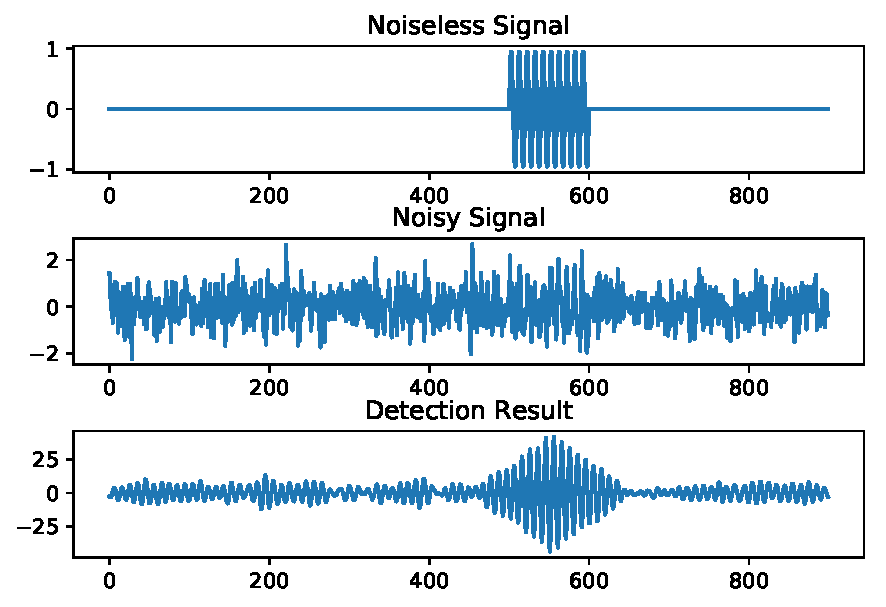
\includegraphics[width=\textwidth]{sinusoidDetection.pdf}}
\end{columns}
\end{frame}

\begin{frame}[allowframebreaks=0.8]
 {Detection of random signals}
\begin{itemize}
\item The problem with the previous approach was that the model was too
restrictive; the results depend on how well the phases match.
\item The model can be relaxed by considering \emph{random signals},
whose exact form is unknown, but the correlation structure is known.
Since the correlation captures the frequency (but not the phase),
this is exactly what we want.
\item In general, the detection of a random signal can be formulated as
follows.
\item Suppose $\s \sim {\cal N}(0, {\bf C}_s)$ and $\w \sim {\cal N}(0, \sigma^2 {\bf I})$.
Then the detection problem is a hypothesis test
\begin{align*}
{\cal H}_0&:  \x\sim{\cal N}(0, \sigma^2 {\bf I})\\
{\cal H}_1&:  \x\sim{\cal N}(0, {\bf C}_s + \sigma^2 {\bf I})
\end{align*}
\item It can be shown, that the decision rule becomes
\[
\text{Decide } {\cal H}_1, \text{ if } \x^T\hat{\s} > \gamma,
\]
where
\[
\hat{\s} = {\bf C}_s({\bf C}_s + \sigma^2 {\bf I})^{-1}\x.
\]
\end{itemize}
\end{frame}

\begin{frame}[allowframebreaks=0.8,fragile]
 {Example of Random Signal Detection}
\begin{itemize}
\item Without going into the details, let's jump directly to the derived decision
rule for the sinusoid:
\[
\left|\sum_{n=0}^{N-1} x[n]\exp(-2\pi i f_0 n) \right| > \gamma.
\]
\item As an example, the below picture shows the detection process with $\sigma = 0.5$.

\item Note the simplicity of Python implementation:
\end{itemize}
\begin{center}
\begin{minipage}{5cm}
\begin{lstlisting}
import numpy as np

h = np.exp(-2 * np.pi * 1j * f0 * n)
y = np.abs(np.convolve(h, xn, 'same'))
\end{lstlisting}
\end{minipage}
\end{center}
\centerline{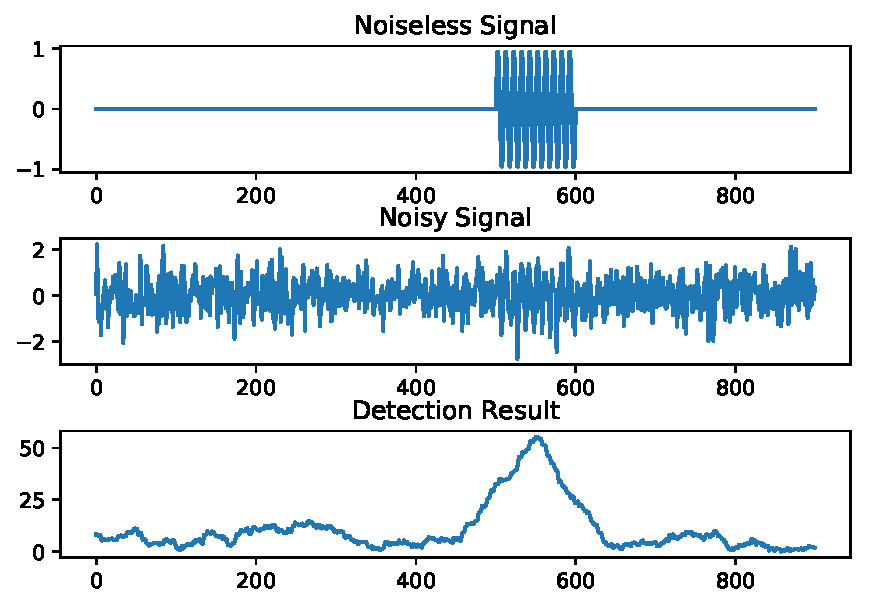
\includegraphics[width=0.65\textwidth]{rayleighSinusoid.pdf}}
\end{frame}



\begin{frame}[fragile,allowframebreaks=0.8]
 {Receiver Operating Characteristics}

\begin{itemize}
\item A usual way of illustrating the detector performance is the
\emph{Receiver Operating Characteristics} curve (ROC curve).
\item This describes the relationship between $P_{FA}$ and $P_D$
for all possible values of the threshold $\gamma$.
\item The functional relationship between $P_{FA}$ and $P_D$
depends on the problem and the selected detector.
\end{itemize}
\end{frame}



\begin{frame}[fragile,allowframebreaks=0.8]
 {Receiver Operating Characteristics}
\begin{columns}
\column{0.65\textwidth}
\begin{itemize}
\item For example, in the DC level example, 
\begin{align*}
P_D(\gamma) = \int_{\gamma}^{\infty} \frac{1}{\sqrt{2\pi}}\exp\left(-\frac{(x-1)^2}{2}\right)\,dx\\
P_{FA}(\gamma) = \int_{\gamma}^{\infty} \frac{1}{\sqrt{2\pi}}\exp\left(-\frac{x^2}{2}\right)\,dx
\end{align*}
\item It is easy to see the relationship:
\[
P_D(\gamma) = \int_{\gamma-1}^{\infty} \frac{1}{\sqrt{2\pi}}\exp\left(-\frac{x^2}{2}\right)\,dx = P_{FA}(\gamma-1).
\]
\item Plotting the ROC curve for all $\gamma$ is shown on the right.
\end{itemize}

\column{0.35\textwidth}
\centerline{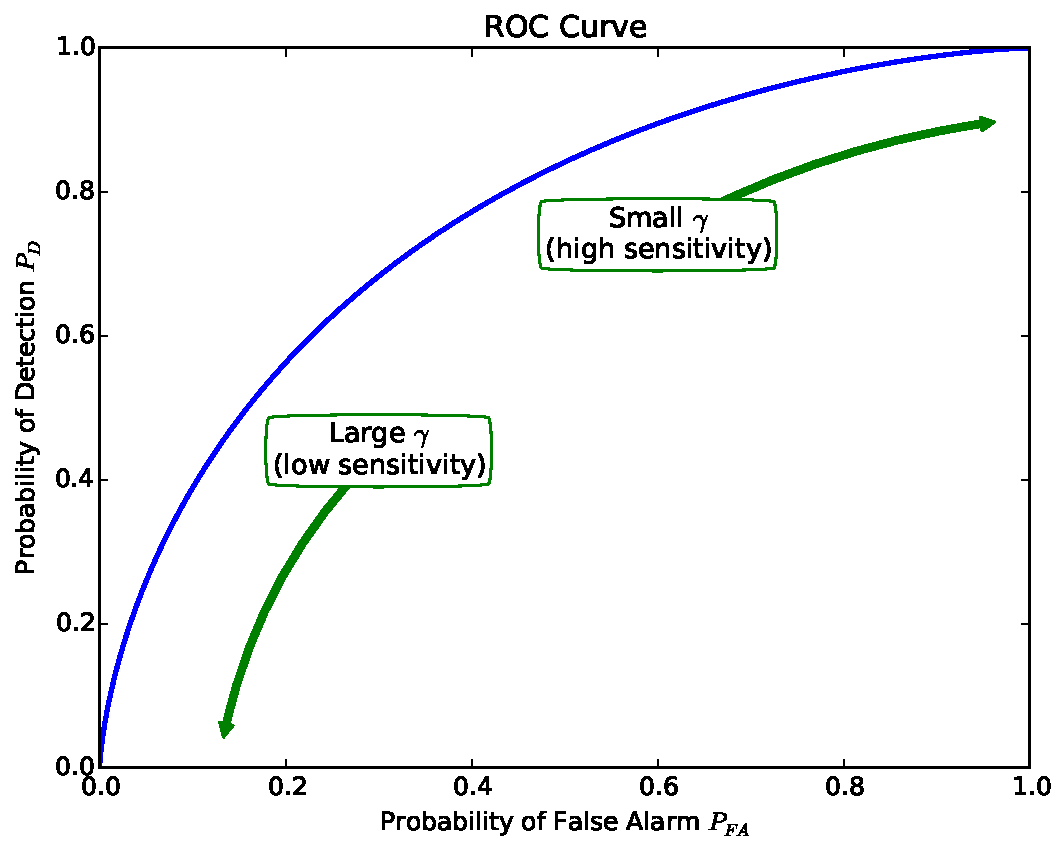
\includegraphics[width=\textwidth]{RocCurve.pdf}}

\end{columns}
%\centerline{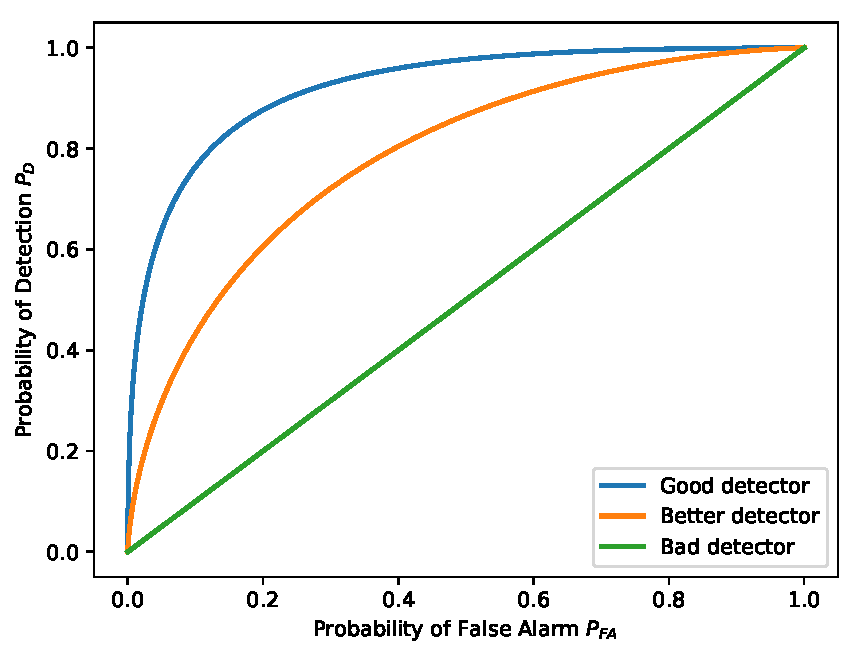
\includegraphics[width=0.5\textwidth]{roc_difficulty.pdf}}

%\centerline{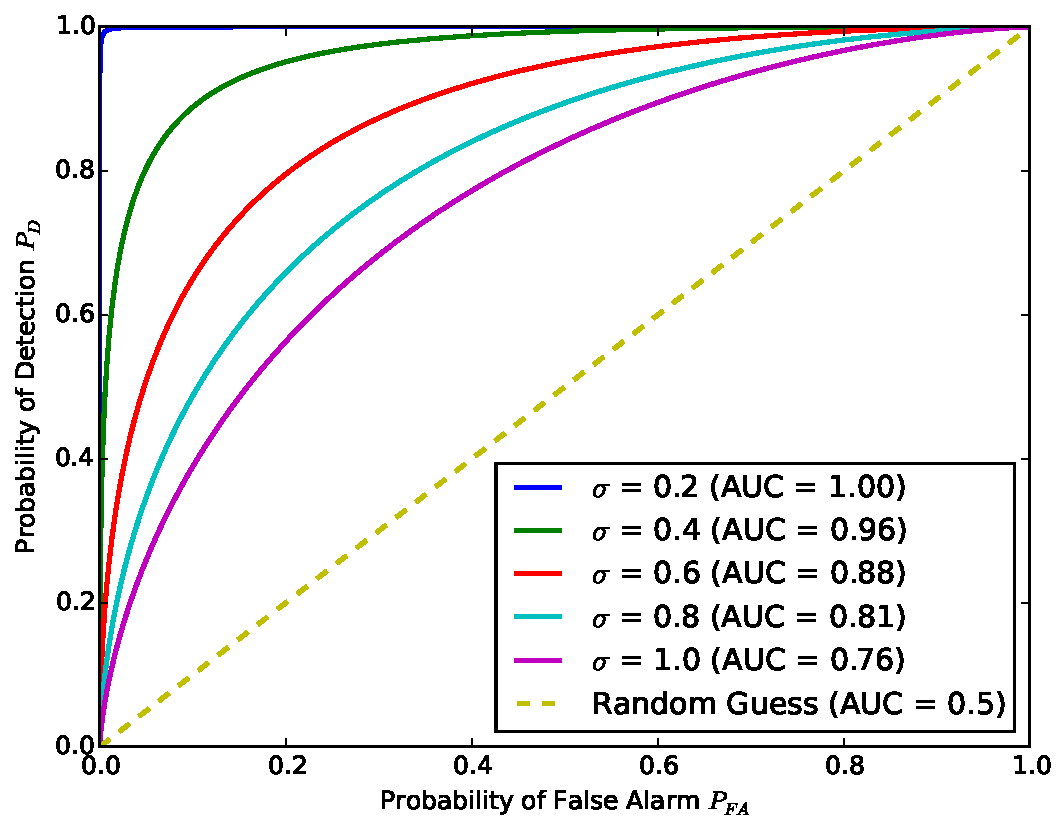
\includegraphics[width=0.5\textwidth]{RocCurve2.pdf}}
\end{frame}


\begin{frame}[fragile,allowframebreaks=0.8]
 {Receiver Operating Characteristics}
\begin{columns}
\column{0.65\textwidth}

\begin{itemize}
\item The higher the ROC curve, the better the performance. 
\item A random guess has diagonal ROC curve.
\item This gives rise to a widely used measure for detector
performance: the \emph{Area Under (ROC) Curve}, or AUC criterion.
\item The benefit of AUC is that it is threshold independent, and tests
the accuracy for \textit{all} thresholds.
%\item In the DC level case, the performance increases if the noise variance $\sigma^2$ decreases (since the 
%problem becomes easier).
%\item Below are the ROC plots for various values of $\sigma^2$.
\end{itemize}

\column{0.35\textwidth}
\centerline{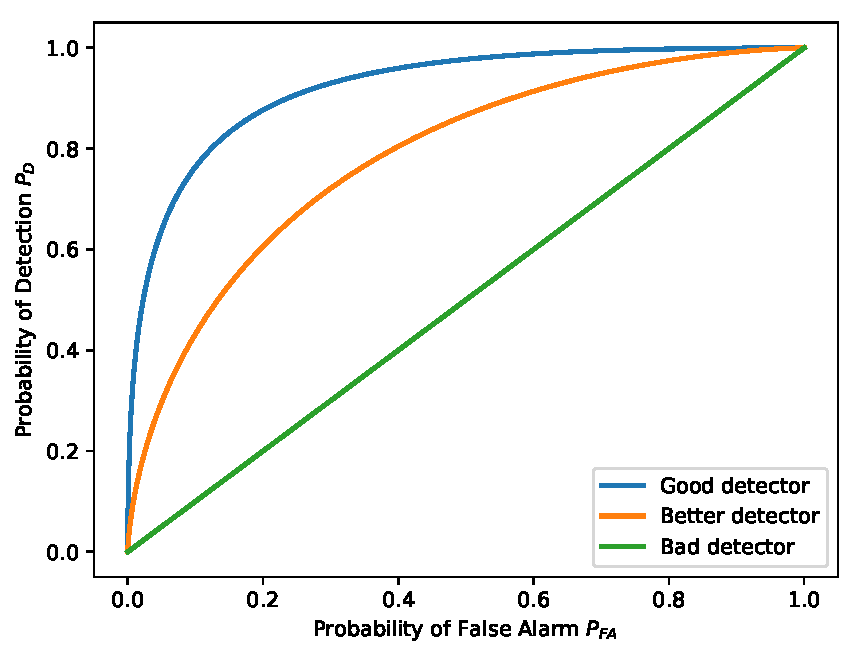
\includegraphics[width=\textwidth]{roc_difficulty.pdf}}

\end{columns}
%\centerline{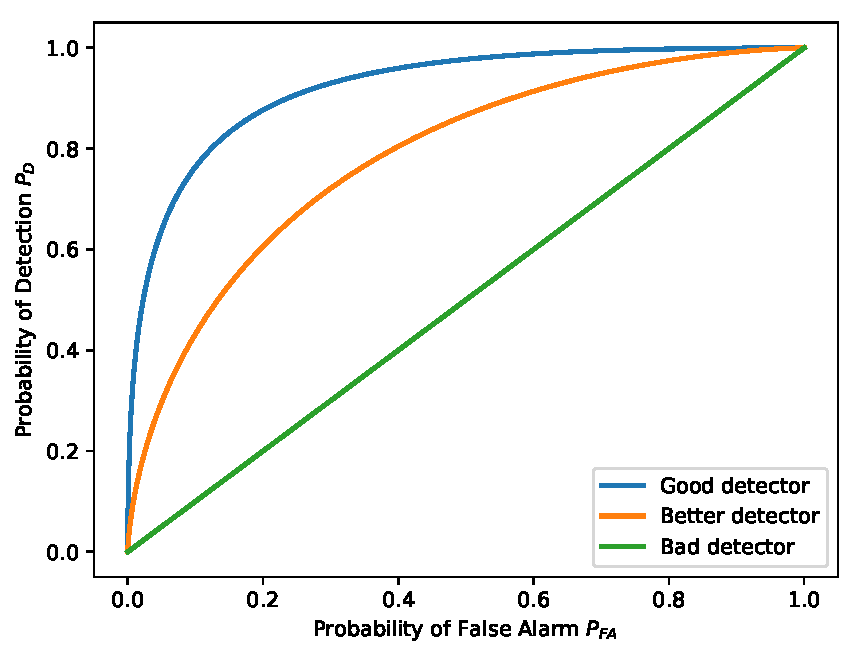
\includegraphics[width=0.5\textwidth]{roc_difficulty.pdf}}

%\centerline{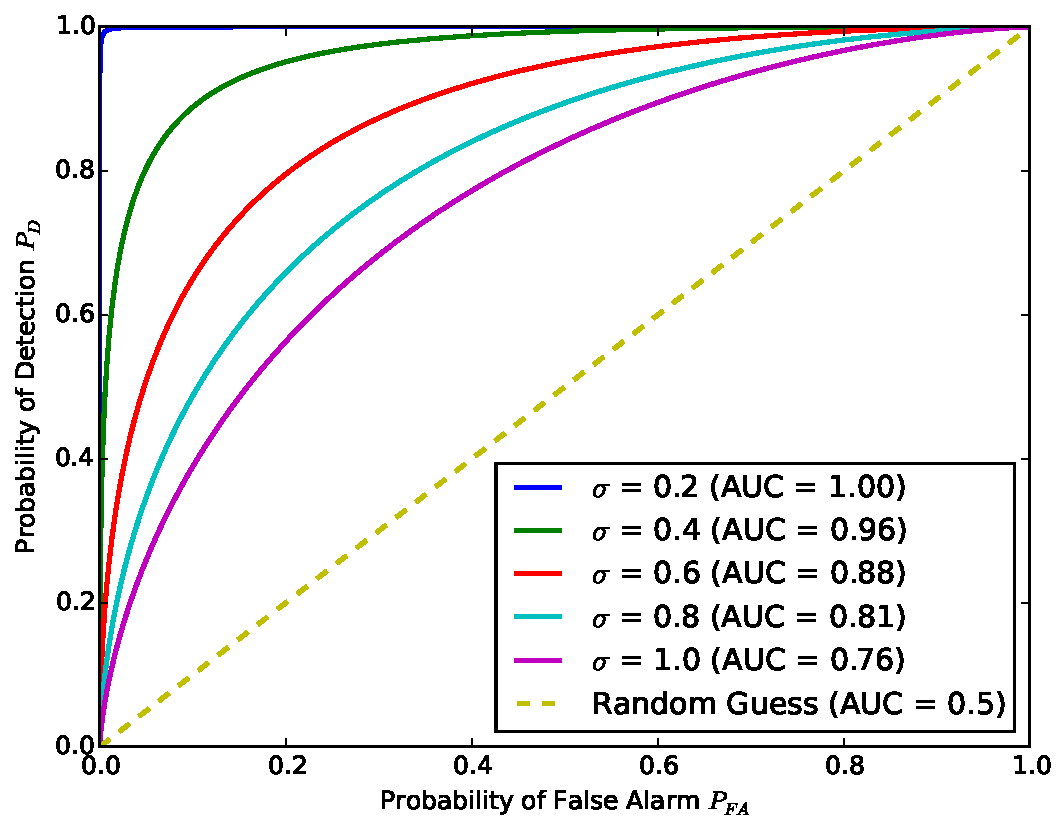
\includegraphics[width=0.5\textwidth]{RocCurve2.pdf}}
\end{frame}

\begin{frame}[allowframebreaks=0.8]
 {Empirical AUC}
\begin{itemize}
\item Initially, AUC and ROC stem from radar and radio detection problems.
\item More recently, AUC has become one of the standard measures of classification performance, as well.
\item Usually a closed form expression for $P_D$ and $P_{FA}$ can not be derived.
\item Thus, ROC and AUC are most often computed empirically;\textit{ i.e.}, by evaluating the prediction results
on a holdout test set.
\end{itemize}
\end{frame}

\begin{frame}{Classification Example---ROC and AUC}
\begin{columns}
\column{0.8\textwidth}
\begin{itemize}
\item For example, consider the 2-dimensional dataset on the right.
\item The data is split to \textit{training} and \textit{test} sets, which
are \textit{similar} but not exactly the \textit{same}.
\item Let's train 4 classifiers on the upper data and compute the ROC 
for each on the bottom data.
\end{itemize}
\column{0.25\textwidth}
\centerline{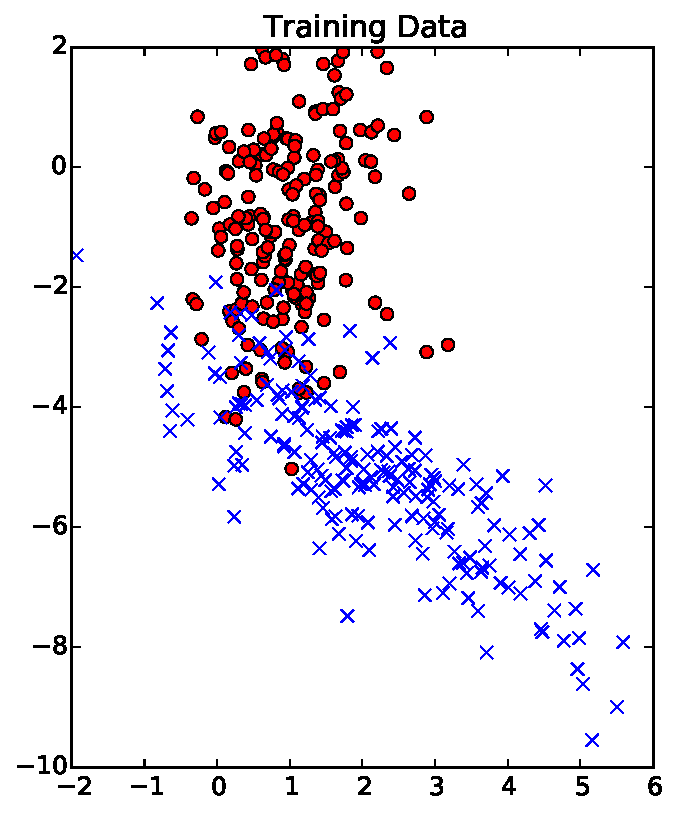
\includegraphics[width=0.8\columnwidth]{TrainingData_2class.pdf}}\\
\centerline{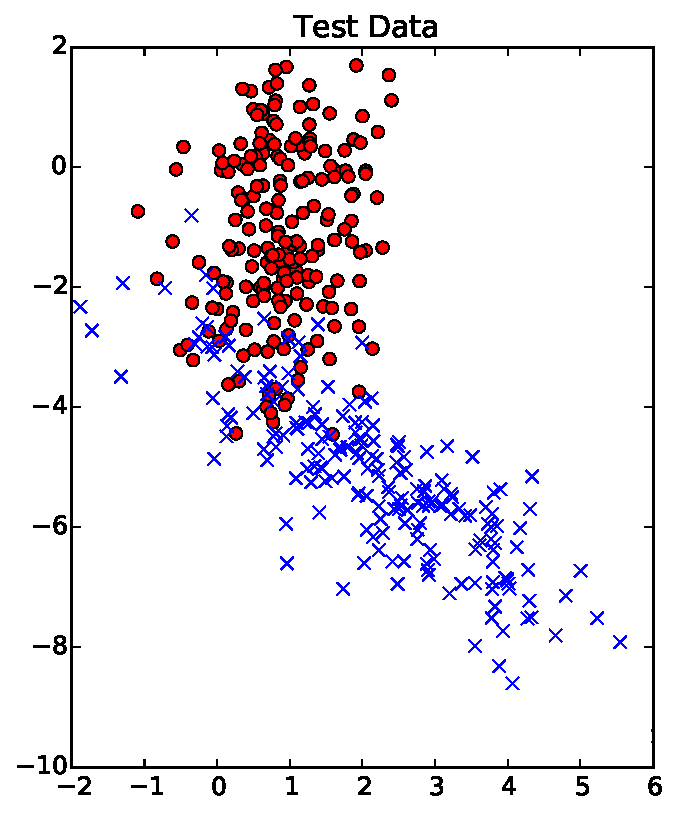
\includegraphics[width=0.8\columnwidth]{TestData_2class.pdf}}
\end{columns}
\end{frame}

\begin{frame}{Classification Example---ROC and AUC}
\begin{columns}
\column{0.65\textwidth}
\begin{itemize}
\item A linear classifier trained with the training data
produces the shown class boundary.
\item The class boundary has the orientation and location 
that minimizes the overall classification error for the training data.
\item The boundary is defined by:
\[
y = c_1 x + c_0
\]
with parameters $c_1$ and $c_0$ learned from data.
\end{itemize}
\column{0.4\textwidth}
\centerline{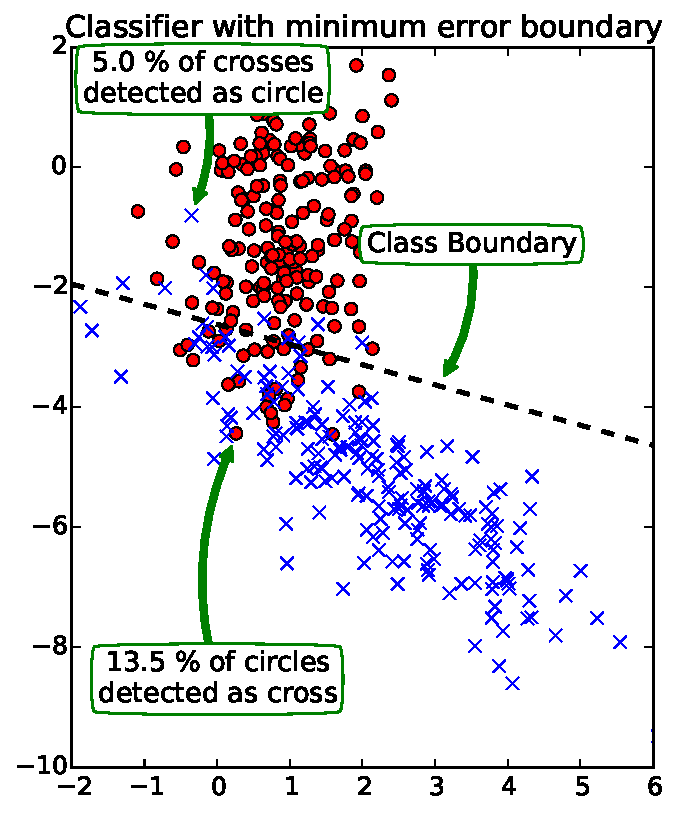
\includegraphics[width=\columnwidth]{2classBoundary.pdf}}
\end{columns}
\end{frame}

\begin{frame}{Classification Example---ROC and AUC}
\begin{columns}
\column{0.8\textwidth}
\begin{itemize}
\item We can adjust the sensitivity of classification by moving the decision boundary up or down.
\item In other words, slide the parameter $c_0$ in 
\[
y = c_1 x + c_0
\]
\item This can be seen as a \textit{tuning parameter} for plotting the ROC curve.
\end{itemize}
\column{0.25\textwidth}
\vspace*{0.5cm}
\centerline{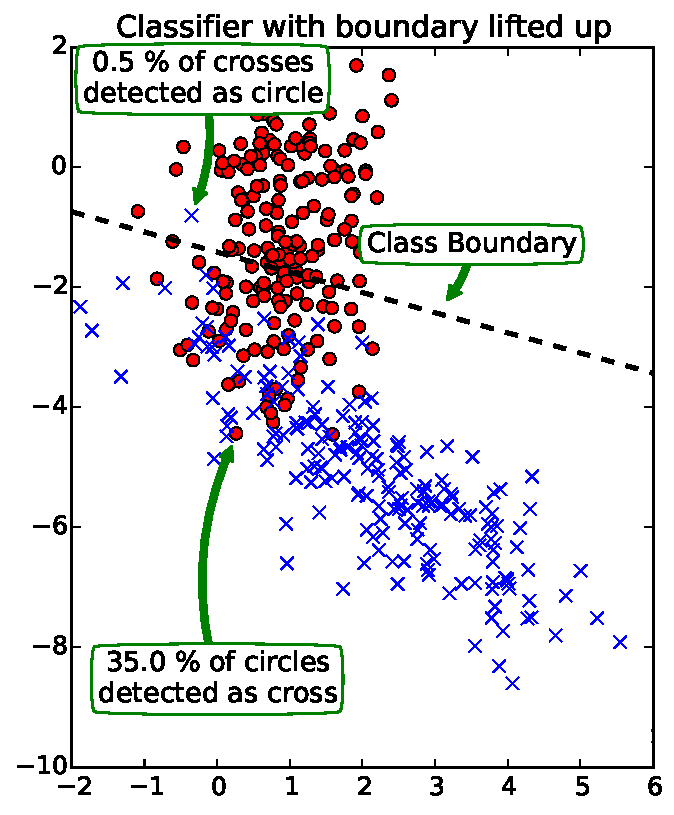
\includegraphics[width=0.8\columnwidth]{2classBoundary_lowSensitivity.pdf}}\\
\centerline{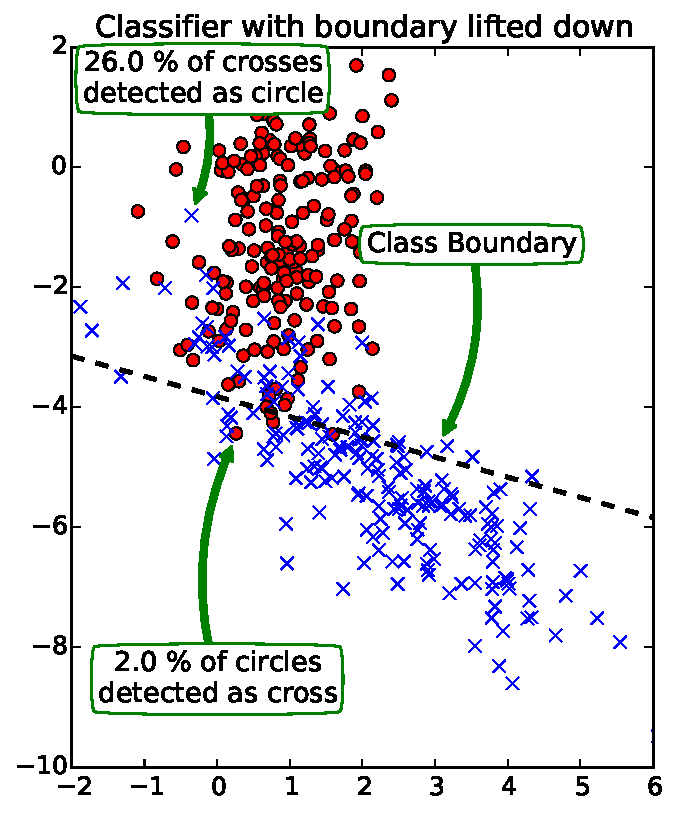
\includegraphics[width=0.8\columnwidth]{2classBoundary_highSensitivity.pdf}}
\end{columns}
\end{frame}

\begin{frame}{Classification Example---ROC and AUC}

\begin{itemize}
\item When the boundary slides from bottom to top, we plot the \textit{empirical ROC curve}.
\item Plotting starts from upper right corner.
\item Every time the boundary passes a blue cross, the curve moves left.
\item Every time the boundary passes a red circle, the curve moves down.
\end{itemize}
\centerline{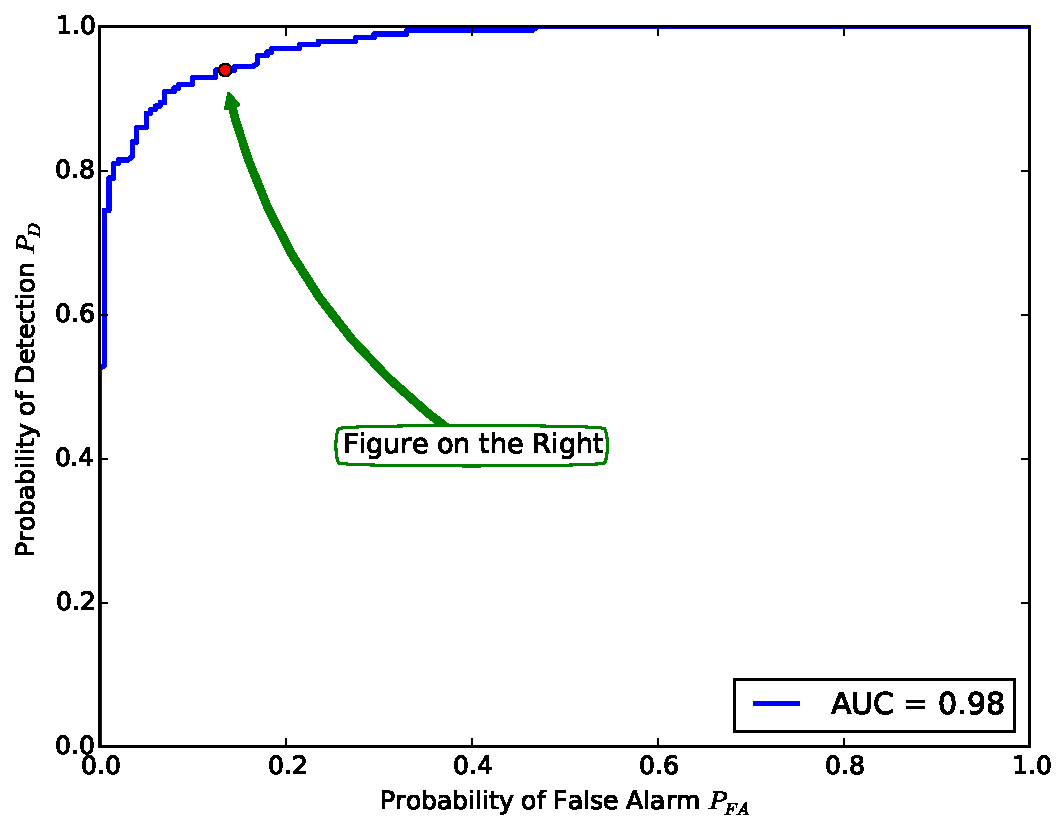
\includegraphics[width=0.4\columnwidth]{2classBoundary_ROC.pdf}
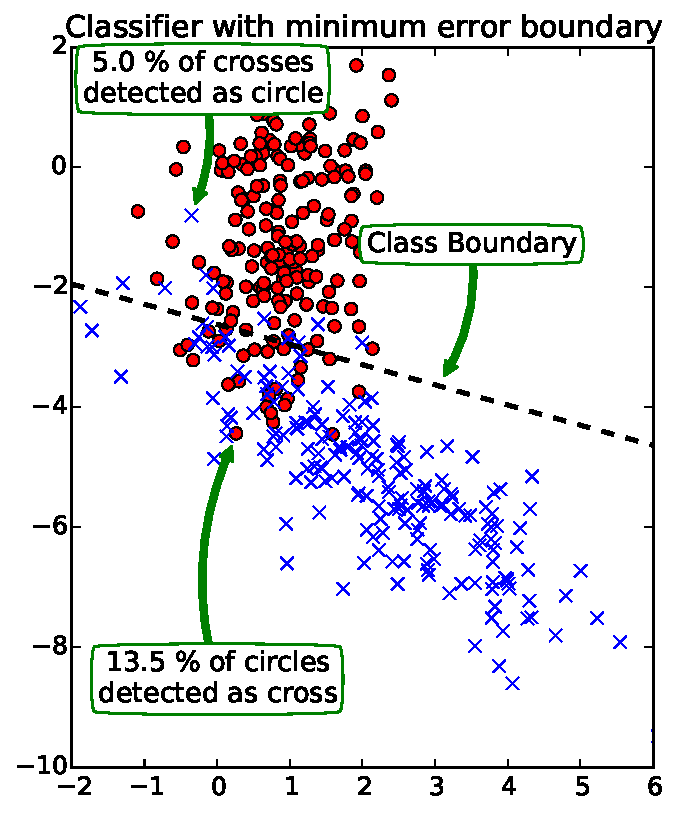
\includegraphics[width=0.27\columnwidth]{2classBoundary.pdf}}
\end{frame}

\begin{frame}{Classification Example---ROC and AUC}

\begin{itemize}
\item Real usage is for comparing classifiers.
\item Below is a plot of ROC curves for 4 widely used classifiers.
\item Each classifier produces a class membership score over which the
tuning parameter slides.
\end{itemize}
\centerline{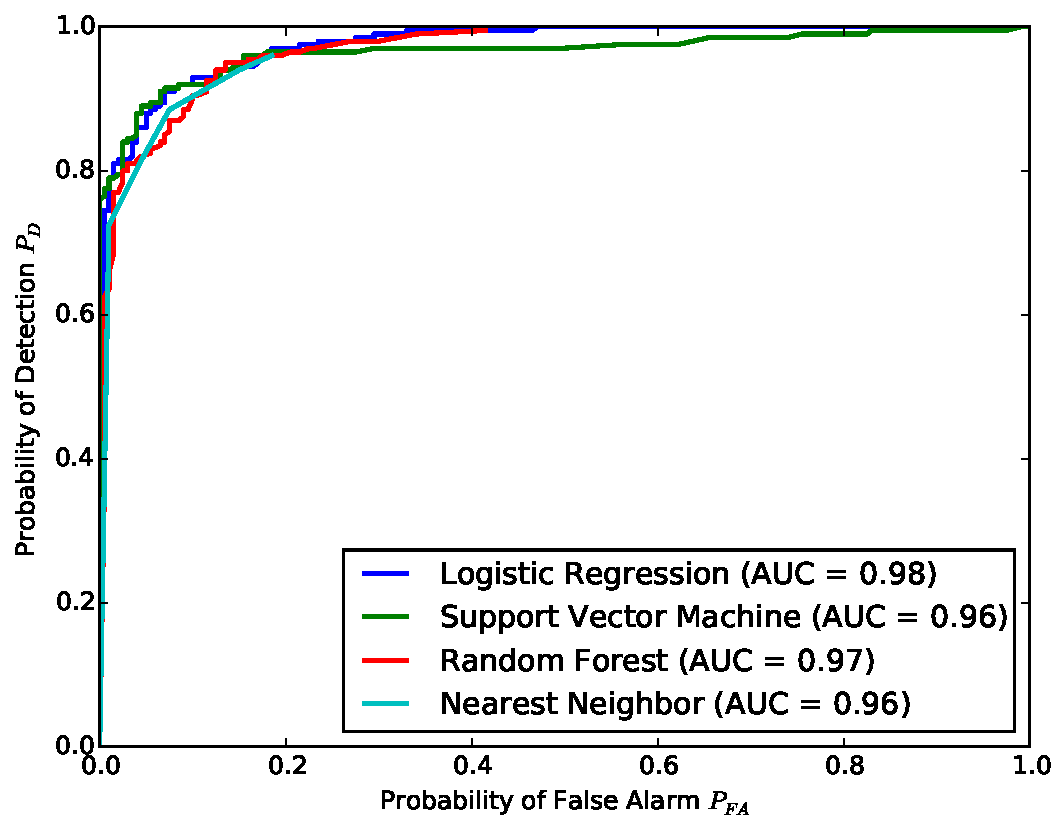
\includegraphics[width=0.4\columnwidth]{2classBoundary_ROC_4clf.pdf}}
\end{frame}

\begin{frame}[allowframebreaks=0.8, fragile]{ROC and AUC code in Python}
\begin{lstlisting}
classifiers = [(LogisticRegression(), "Logistic Regression"),
               (SVC(probability = True), "Support Vector Machine"),
               (RandomForestClassifier(n_estimators = 100), "Random Forest"),
               (KNeighborsClassifier(), "Nearest Neighbor")]
        
for clf, name in classifiers:
    clf.fit(X, y)
    
    ROC = []
    for gamma in np.linspace(0, 1, 1000):
        
        err1 = np.count_nonzero(clf.predict_proba(X_test[y_test == 0, :])[:,1] <= gamma)
        err2 = np.count_nonzero(clf.predict_proba(X_test[y_test == 1, :])[:,1] > gamma)
    
        err1 = float(err1) / np.count_nonzero(y_test == 0)
        err2 = float(err2) / np.count_nonzero(y_test == 1)
        
        ROC.append([err1, err2])
    ROC = np.array(ROC)
    
    ROC = ROC[::-1, :]
    auc = roc_auc_score(y_test, clf.predict_proba(X_test)[:,1])
    
    plt.plot(1-ROC[:, 0], ROC[:, 1], linewidth = 2, label="%s (AUC = %.2f)" % (name, auc))
\end{lstlisting}
\vspace*{-1cm}
\end{frame}
%
%\begin{frame}[allowframebreaks=0.8]
 %{Composite hypothesis testing}
%\begin{itemize}
%\item In the previous examples the parameter values specified the
%distribution completely; e.g., either $A=1$ or $A=0$.
%\item Such cases are called \emph{simple hypotheses testing}.
%\item Often we can't specify exactly the parameters for either case,
%but instead a range of values for each case.
%\item An example could be our DC model $x[n] = A + w[n]$ with
%\begin{align*}
%{\cal H}_1 &: A \ne 0\\
%{\cal H}_0 &: A = 0
%\end{align*}
%
%\item The question can be posed in a probabilistic manner as follows:
%\\
%\medskip
%
%{\em What is the probability of observing $x[n]$ if ${\cal H}_0$ would hold?}
%\medskip
%
%\item If the probability is small (e.g., all $x[n]\in [0.5,1.5]$, and
%let's say the probability of observing $x[n]$ under ${\cal H}_0$ is 1 \%), 
%then we can conclude that the null hypothesis can be \emph{rejected} with
%99\% confidence.
%
%\end{itemize}
%
%\end{frame}
%
%
%\begin{frame}[allowframebreaks=0.8]
 %{An example}
%\begin{itemize}
%\item As an example, consider detecting a biased coin in a coin
%tossing experiment. 
%\item If we get 19 heads out of 20 tosses, it seems rather likely that the
%coin is biased.
%\item How to pose the question mathematically?
%\item Now the hypotheses is
%\begin{align*}
%{\cal H}_1 &: \text{coin is biased: } p \ne 0.5 \\
%{\cal H}_0 &: \text{coin is unbiased: } p = 0.5,
%\end{align*}
%where $p$ denotes the probability of a head for our coin.
%\item Additionally, let's say, we want 99\% confidence for 
%the test.
%\item Thus, we can state the hypothesis test as: "what is the
%probability of observing at least 19 heads assuming $p=0.5$?"
%\item This is given by the binomial distribution 
%\[
%\underbrace{{20 \choose 19} 0.5^{19} \cdot 0.5^1}_{\text{19 heads}} 
%\underbrace{+}_{\text{or}} \underbrace{0.5^{20}}_{\text{20 heads}} \approx
%0.00002.
%\]
%\item Since 0.00002 < 1\%, we can reject the null hypothesis and
%the coin is biased.
%\item Actually, the 99\% confidence was a bit loose in this case.
%\item We could have set a 99.98\% confidence requirement and
%still reject the null hypothesis.
%\item The upper limit for the confidence (here 99.98\%) is widely 
%used and called the {\em p-value}.
%\item More specifically,\\ \medskip
%
%\emph{The p-value is the probability of obtaining a test statistic at least as extreme as the one that was actually observed, assuming that the null hypothesis is true.}
%
%\end{itemize}
%
%\end{frame}

\end{document}

